\section{Final architecture}
The final architecture, shown in Figure~\ref{fig:arch-final}, was as a whole relatively similar to our planned architecture. 

\begin{figure}[tbph]
  \centering
  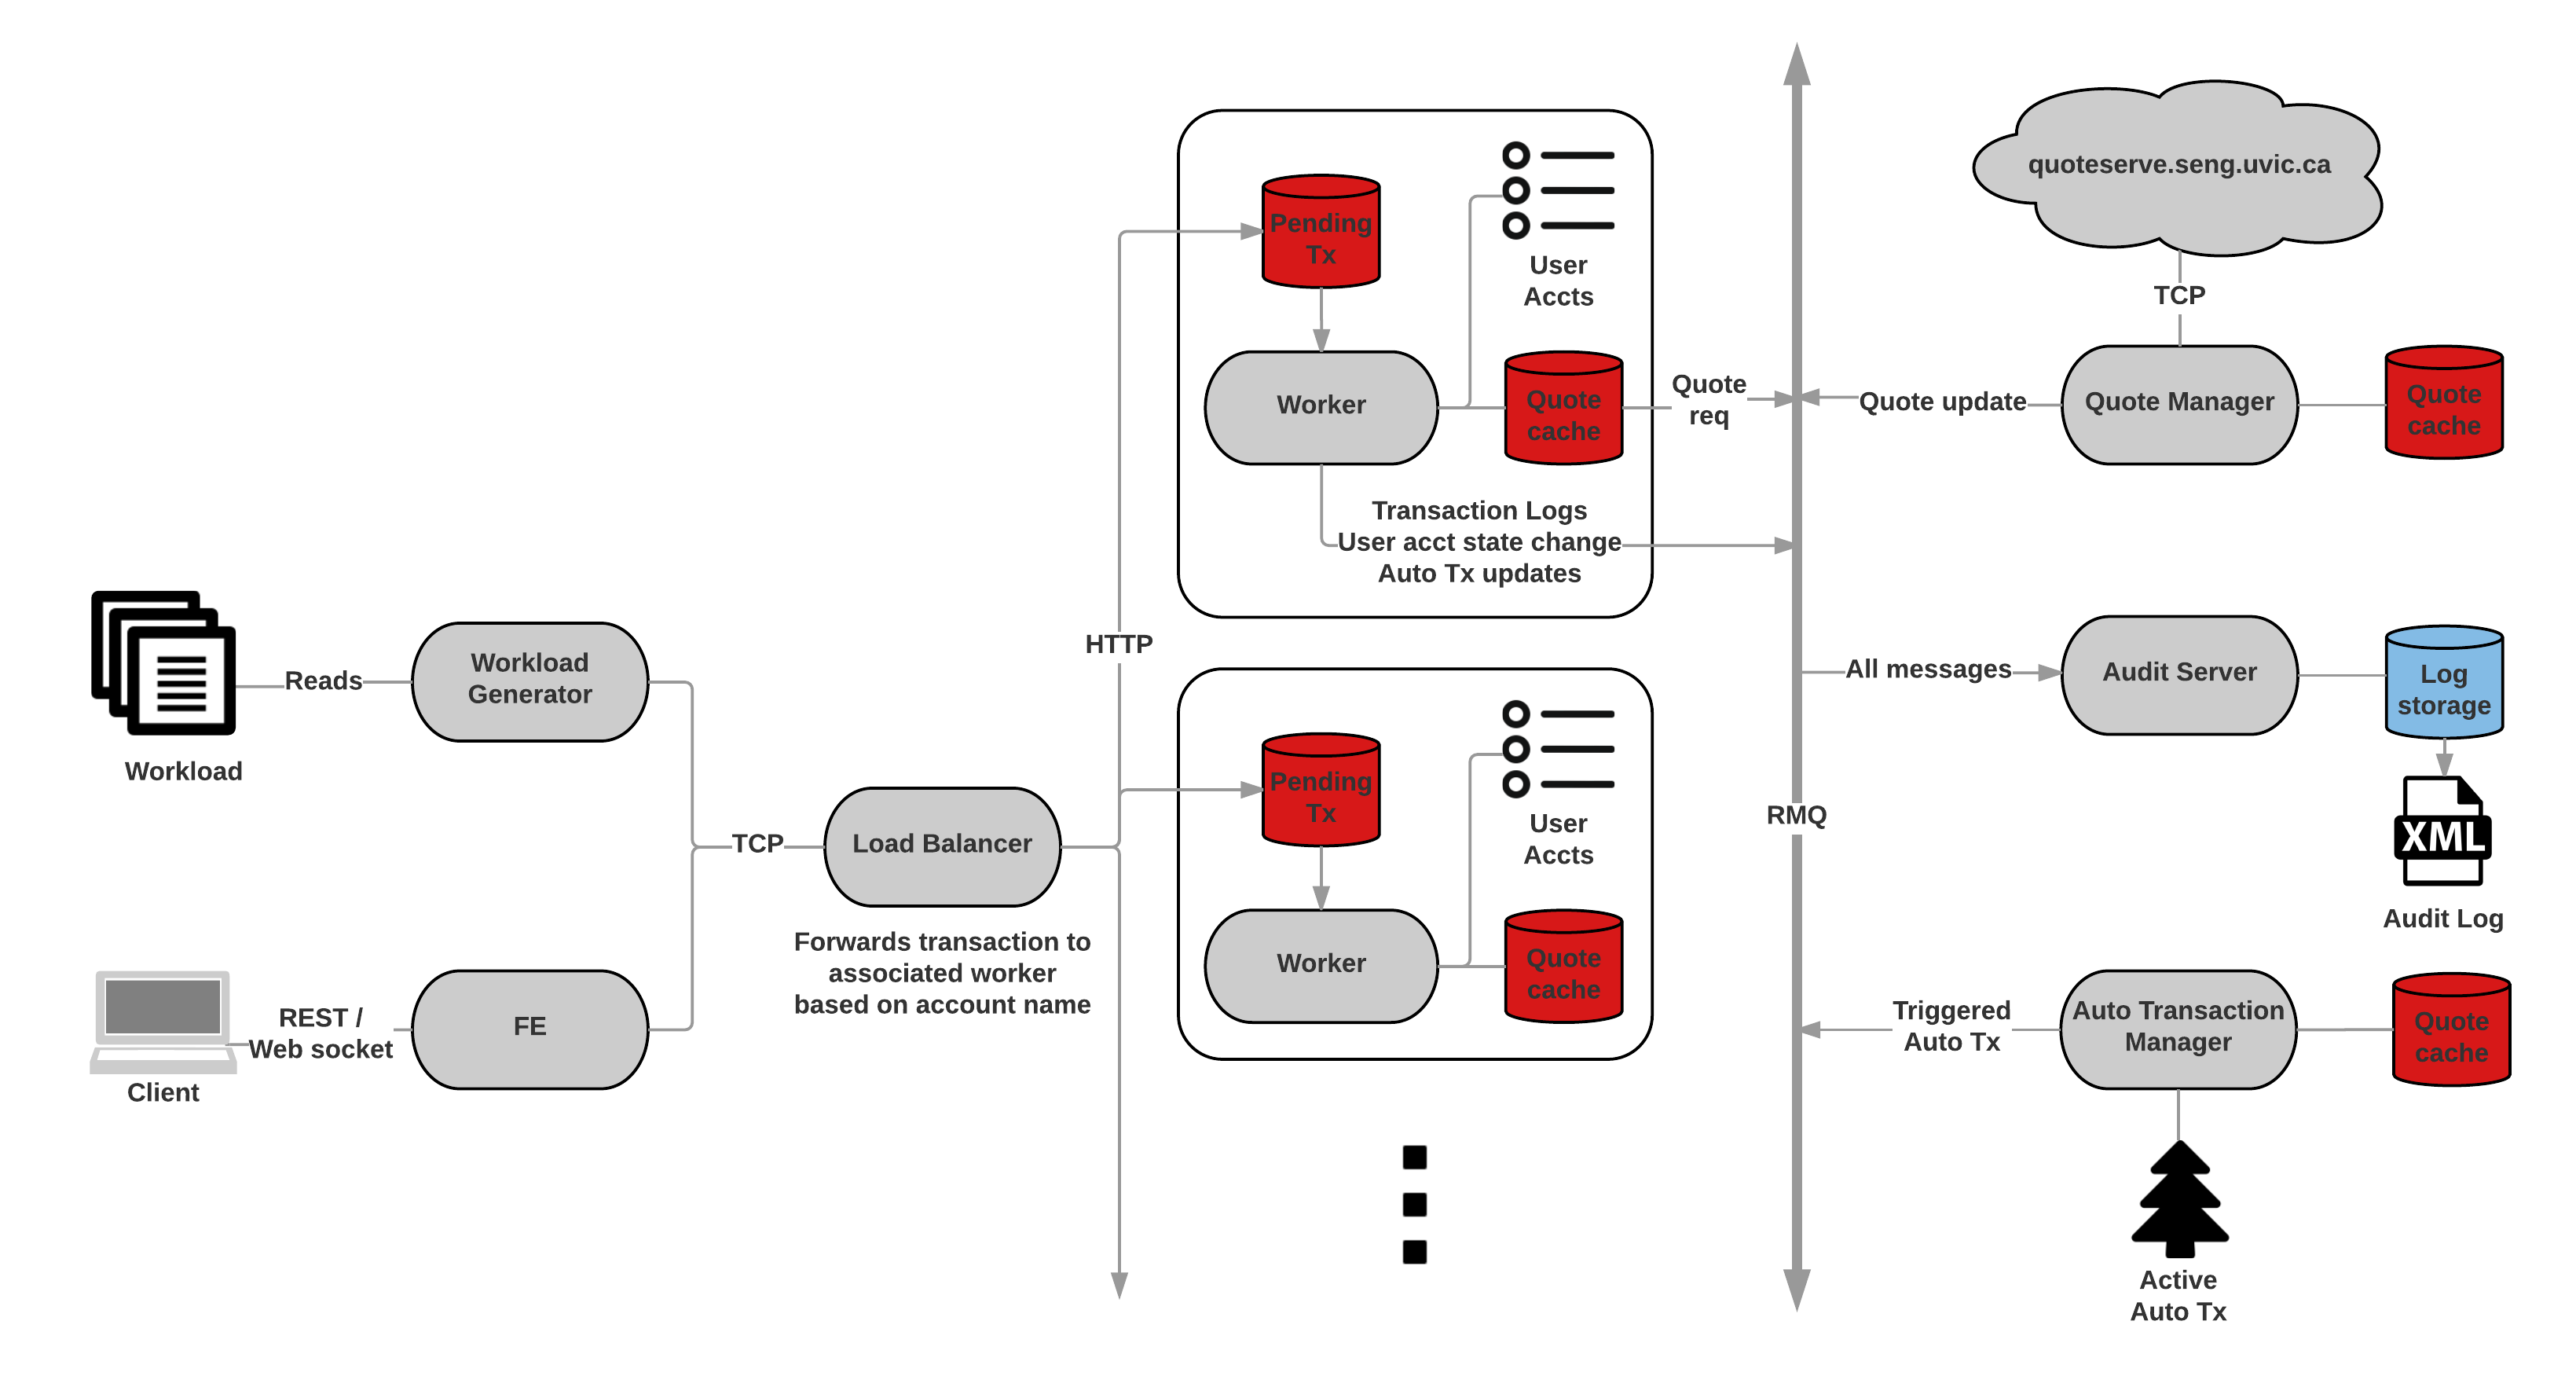
\includegraphics[width=0.85\linewidth]{graphics/arch-final}
  \caption[Final system architecture]{Final system architecture. Red databases are Redis caches, blue databases are Postgres.}
  \label{fig:arch-final}
\end{figure}

\subsection{Incoming traffic}
The method of load balancing had to be modified to account for serving of the frontend and connection of the websockets. Request which enter the load balancer are given a session token, and are always routed back to the same worker. This allows us to skip the microservice which would be responsible for serving an ACID database of userdata. The root url serves an HTML page, which contains the login/create page if a user has not registered. Once at this page, a user is able to register/login, at which point a socket connection will be made to the backend. This socket connection will serve to asynchronously return the account state, as well as any output messages that need to be presented to the user. We opted for an entirely event based pattern instead of trying to modify a request/response style page loading to fit the event system on the backend. This allows all of our requests to be non blocking, and for the user to have the most up to date information all the time.

\subsection{Frontend}
The frontend consists of an authentication screen, and a loggedin view. Each action results in a post request getting sent to the API. Login maps to the \texttt{/login} API endpoint, create maps to the \texttt{/create} API endpoint, and all other actions map to the \texttt{/push} API endpoint. Login and create are responsible for user authentication. Once this is completed, the frontend also requests a consistent websocket connection over the \texttt{/ws} API endpoint. This websocket connection is added to the socket hub on the backend. Any time an event is completed on the backend, the socket hub returns the user’s socket connection and the event is fired over the socket to the users frontend. Each response contains two portions of data: The updated user state, and a message to display on the output screen. The updated user state is parsed on the frontend and displayed to the user.

\subsection{Worker}
The worker as a whole functioned relatively similar to the intended architecture. It stores account data, a local quote cache, and is the workhorse of the entire distributed system.

\subsubsection{Account store}
Accounts are stored on the worker in memory. Each worker is responsible for a sectioning of accounts. Once a user has created an account on a worker, all of it’s incoming requests will be routed through that worker until the account is terminated. While an in memory solution may not seem fault tolerant, all of the events are logged to an audit server, which can be used to replay events on another worker should the original worker crash or go down. In the case of total system failure, the audit logger uses a persistent storage, Postgres, and the system could be brought online simply be replaying all of the transactions from when the audit logger was last live, to when it last went dark.

\subsubsection{Worker goroutines}
The worker ended up divided into seven goroutines. Golang goroutines can be thought of simply as threads or processes which are time sliced.

\paragraph{\texttt{incomingTxWatcher}}
This was responsible for the http setup of the websocket handshaking, the frontend serving, as well as the \texttt{/push} API spinup.

\paragraph{\texttt{sendAutoTx}}
This goroutine spins up and pulls from two channels: \texttt{autoTxInitChan} and \texttt{autoTxCancelChan}. When a user correctly produces an auto transaction by setting and amount and then a trigger value, it is pushed into the channel and pulled by this go routine. In the case of an \texttt{autoTxInit}, we verify the local quote cache to determine if we can fire the trigger instantly, without the help of the autoTx manager.

If the trigger is valid already, it is fulfilled without leaving the worker. If not, we simply publish it to the autoTx manager through its initialization autoTx RMQ.

\texttt{AutoTxCancel} works similarly, except any cancel requests are simply sent straight to the worker. No trigger check is done, since there is no trigger check to do for a cancel.

\paragraph{\texttt{receiveAutoTx}}
This goroutine is the sister routine to \texttt{sendAutoTx}. \texttt{AutoTxFilled} types are sent back to the workers \texttt{autoTxQueue}, which is an RMQ direct exchange where the routing key is the worker ID. When these filled requests come in, they contain an \texttt{AutoTxKey}, an \texttt{AddStock}, and an \texttt{AddFunds}. The idea of this is that both buys and sells can be consumed on the same type, as the result of a buy is an amount of stock, and a remainder of cash, and the result of sell is an amount of stock (0) and a remainder of cash. By unifying these two types, its possible to eliminate the forking behavior that would exist otherwise.

\paragraph{\texttt{catchQuoteBroadcasts}}
This goroutine is relatively simple, as it simply consumes from the quote broadcast exchange and caches the quote into the workers quote cache.

\paragraph{\texttt{fetchNewTx}}
This goroutine is responsible for consuming operations out of the the workers Redis queue and pushing them into the \texttt{unprocessedTx} channel, which is then pulled from by the \texttt{txWorker}.

\paragraph{\texttt{txWorker}}
This goroutine is responsible for the brunt of the processing which occurs on the worker. Whenever an unprocessed transaction is pushed into the \texttt{unprocessedTx} channel, it is then processed by this worker. The command is then parsed into a command object, which contains an execute function based on which type of transaction it is. For example, add transactions will execute the add command in the backend.

\paragraph{\texttt{cleanAccountStore}}
Wakes every sixty seconds to remove expired buys and sells from all user accounts. This prevents the memory loss associated with a user who initiates a large amount of buys or sells but never confirms those actions.

\subsection{Quote manager}
Quote updates involve every part of the distributed system and are the best demonstration of the efficiency of event-sourced architecture. With event-sourcing, each service is free to define its own actions to events that occur in other parts of the system. Figure~\ref{fig:arch-quotes} shows a typical quote request process.

\begin{figure}[tbph]
  \centering
  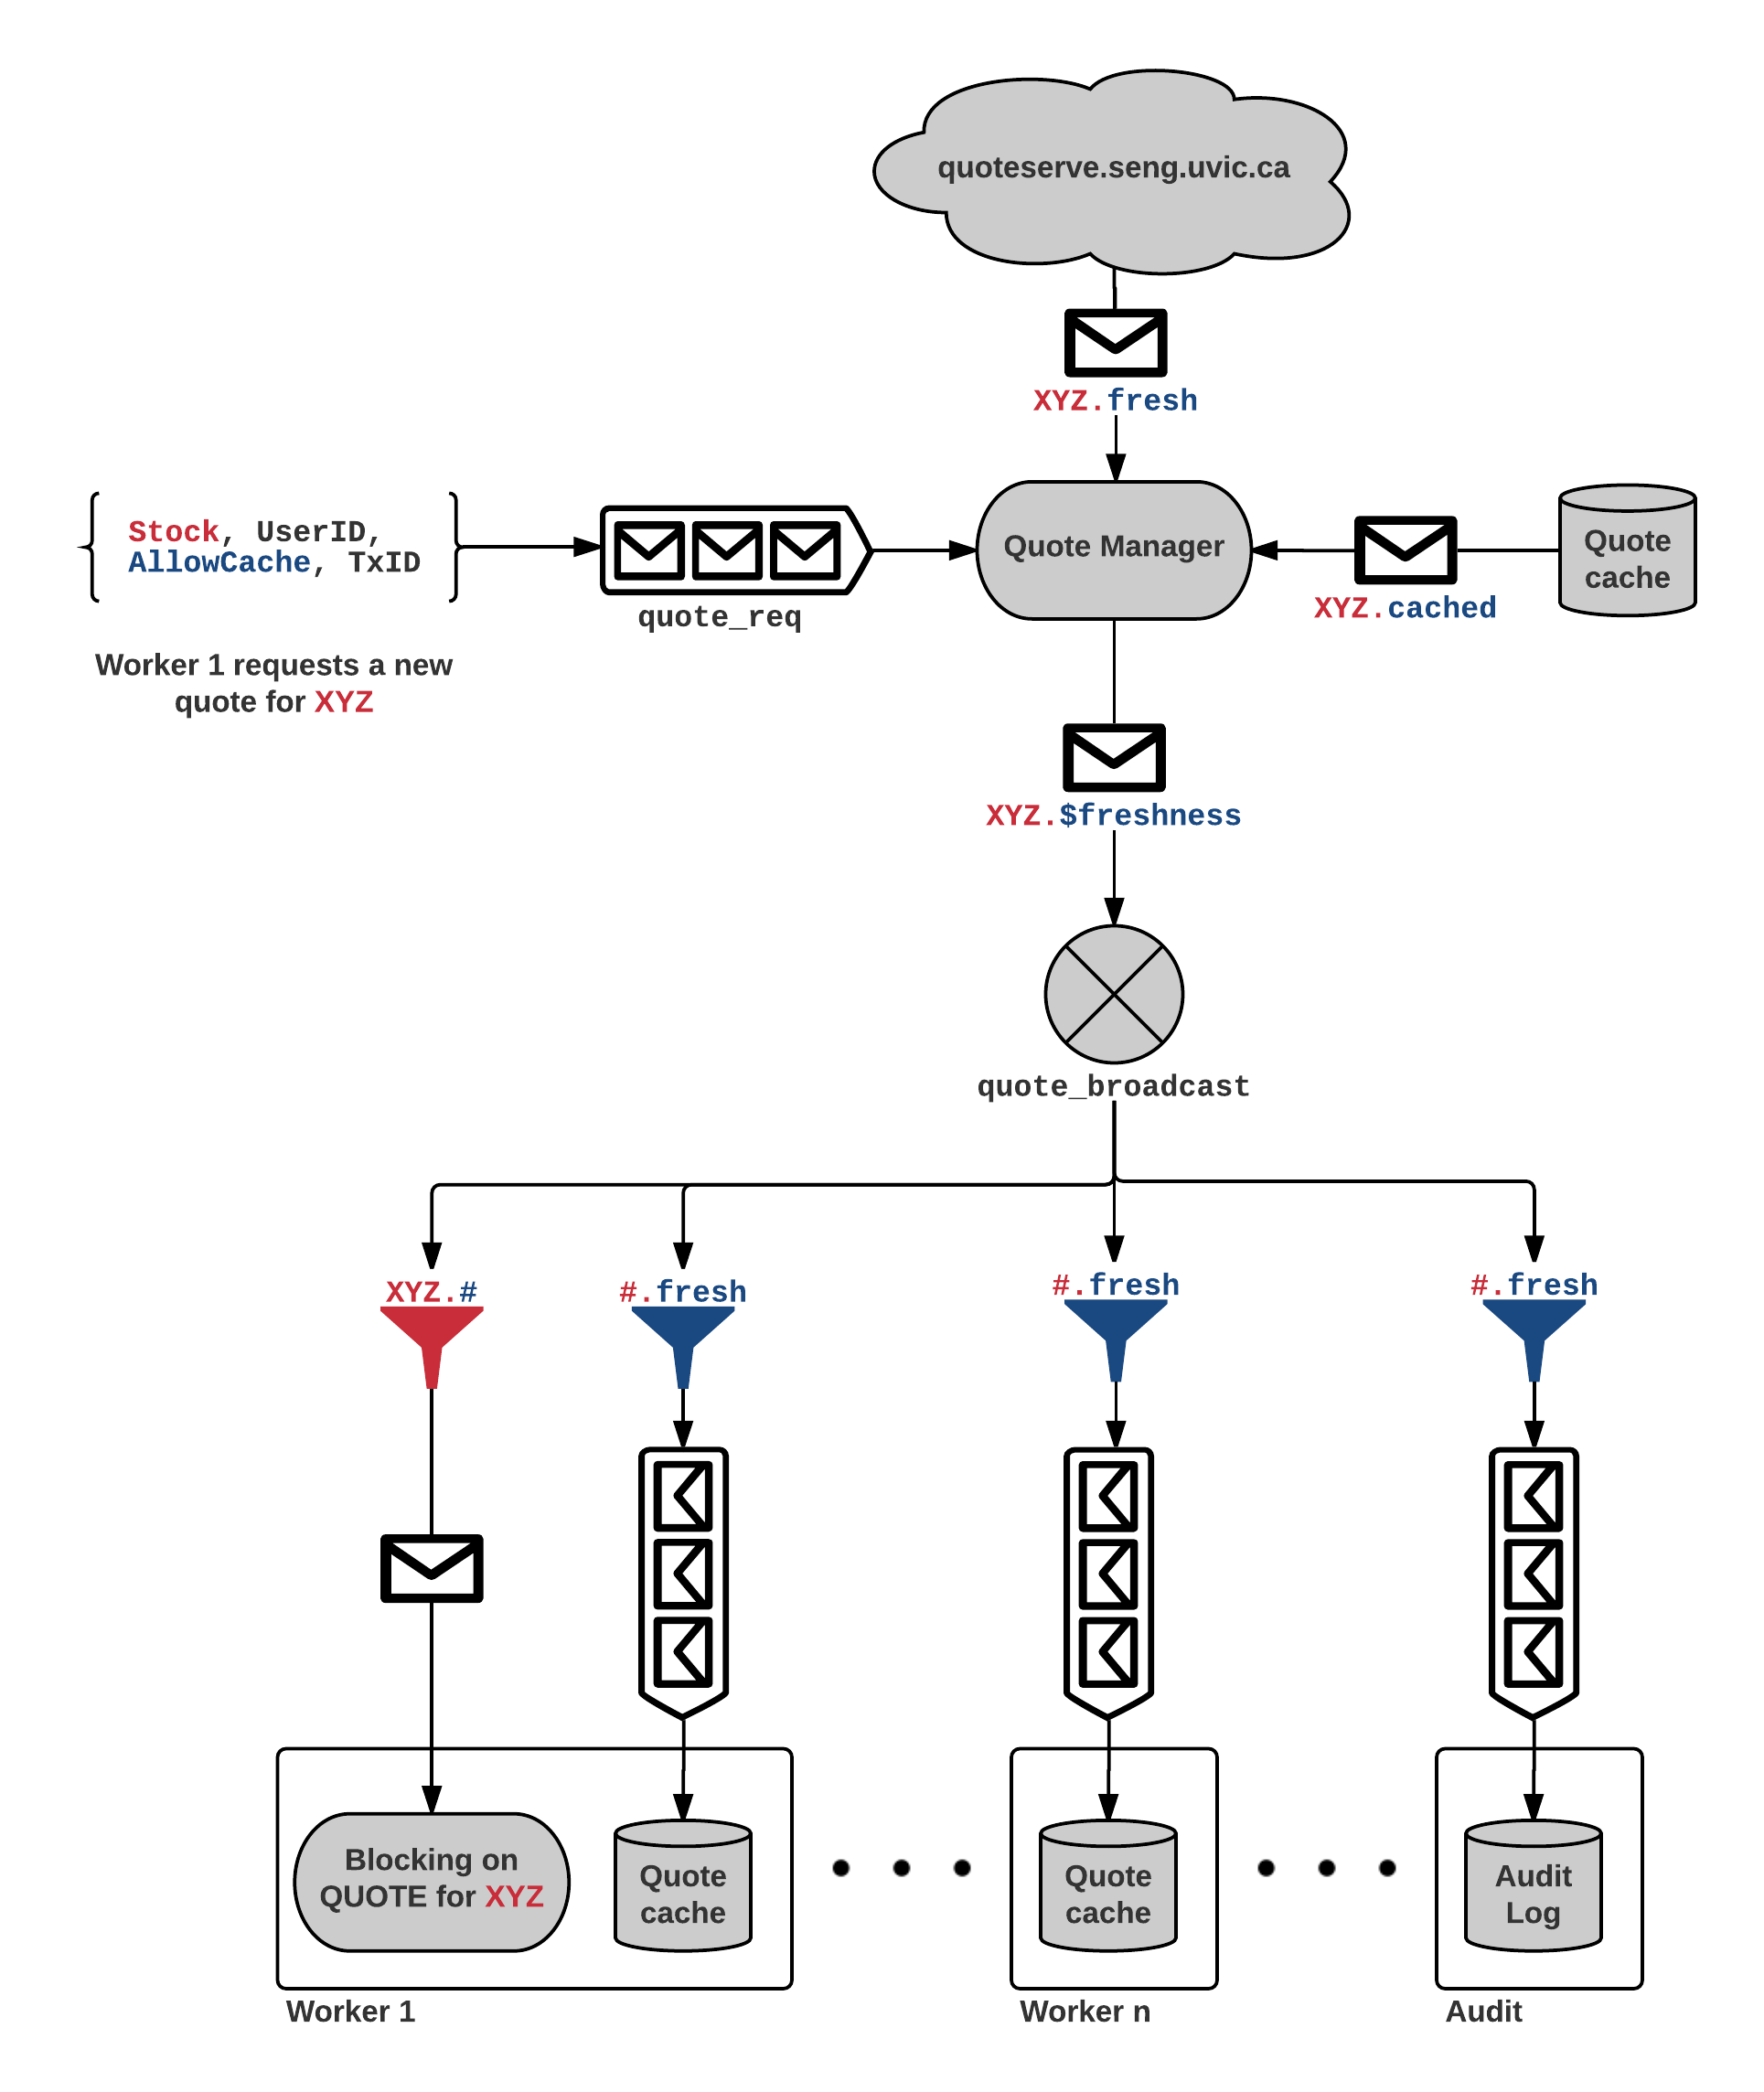
\includegraphics[width=0.85\linewidth]{graphics/arch-quotes}
  \caption{Service interactions for fulfilling a quote}
  \label{fig:arch-quotes}
\end{figure}

Workers generate requests for new quotes, specifying a stock and whether a cached response is allowed. (A \textsc{Buy} for a stock whose quote is about to expire can force a the retrieval of a fresh quote instead of passing the stale quote to the user.) The Quote manager pulls requests from \texttt{quote\_req} RMQ queue and checks for a cached value. On a cache miss, or when forced by a worker, a new quote is requested from the legacy service using the timeout procedure detailed in~\ref{sec:timeout-effectiveness}.

Quotes are broadcast with a key consisting of the stock name and whether the quote was retrieved from a cache or from the legacy service (referred to as ``cached'' and ``fresh'' respectively). Each part of the system filters broadcast messages for its particular purpose. Workers and AutoTX managers need to maintain a local quote cache so they filter ``fresh'' quotes for cache updates. The Audit Logger records quote requests for billing with the same filter. The worker that generated the original request filters for the stock name. This allows two workers to request and block on updates for the same quote and race their requests. Both workers would resume execution when the first quote resolves.


\subsection{Audit logger}
The audit logger required significant redesign in order to accommodate high throughput logging. Section~\ref{sec:log-buf} gives a thorough overview of the necessity of this design and its limitations.

\subsection{AutoTX manager}
The auto transaction manager was designed to be a central point where transactions could be confirmed and sent back to the respective workers. \texttt{AutoTxInit} messages are sent from the worker containing an \texttt{AutoTxKey} (\texttt{Stock}, \texttt{UserID}, \texttt{Action}) as well as an amount and a trigger. \texttt{AutoTxInit} objects are taken and inserted into an AutoTxStore, which contains a map of all \texttt{autoTxKeys} to \texttt{autoTxInits} (For cancellation of transactions), and a map of \texttt{TreeKeys} (\texttt{Stock}, \texttt{Action}) which maps a \texttt{Stock} and \texttt{Action} to a \texttt{Tree}. When multiple auto transaction buys for a stock ABC comes in, they are inserted into a left leaning red black tree. A red black tree was chosen because it excels at heavy read/write workloads and it is self balancing. The auto transaction manager is responsible for requesting quote updates for each stock which resides in it’s store.

The auto transaction manager is also subscribed to the same quote broadcast exchange as the other workers. When a new quote comes in, the buy and sell trees for that stock are observed. It is very simple to partition the tree into fillable transactions and unfillable transactions, because red black trees are binary search trees and are balanced and ordered by their very nature. For each fired trigger, the node is removed from both the tree and the map and then the \texttt{AutoTxFilled} transaction is sent back to the worker which instantiated it.

When \texttt{autoTxCancels} arrive at the autoTx manager, they are simply removed from the autoTx store.

While the auto transaction manager is the only place where user data meets, user data will never interact with any other user data, as comparisons are only done between the quote value and the amount specified by the user. This ensures no cross contamination of data, or mismatching of auto transactions.

